%%%%%%%%%%%%%%%%%%%%%%%%%%%%%%%%%%%%%%%
% Wenneker Resume/CV
% LaTeX Template
% Version 1.1 (19/6/2016)
%
% This template has been downloaded from:
% http://www.LaTeXTemplates.com
%
% Original author:
% Frits Wenneker (http://www.howtotex.com) with extensive modifications by 
% Vel (vel@LaTeXTemplates.com)
%
% License:
% CC BY-NC-SA 3.0 (http://creativecommons.org/licenses/by-nc-sa/3.0/
%
%%%%%%%%%%%%%%%%%%%%%%%%%%%%%%%%%%%%%%

%----------------------------------------------------------------------------------------
%	PACKAGES AND OTHER DOCUMENT CONFIGURATIONS
%----------------------------------------------------------------------------------------

\documentclass[a4paper,12pt]{memoir} % Font and paper size

%%%%%%%%%%%%%%%%%%%%%%%%%%%%%%%%%%%%%%%%%
% Wenneker Resume/CV
% Structure Specification File
% Version 1.1 (19/6/2016)
%
% This file has been downloaded from:
% http://www.LaTeXTemplates.com
%
% Original author:
% Frits Wenneker (http://www.howtotex.com) with extensive modifications by 
% Vel (vel@latextemplates.com)
%
% License:
% CC BY-NC-SA 3.0 (http://creativecommons.org/licenses/by-nc-sa/3.0/)
%
%%%%%%%%%%%%%%%%%%%%%%%%%%%%%%%%%%%%%%%%%

%----------------------------------------------------------------------------------------
%	PACKAGES AND OTHER DOCUMENT CONFIGURATIONS
%----------------------------------------------------------------------------------------

\usepackage{XCharter} % Use the Bitstream Charter font
\usepackage[utf8]{inputenc} % Required for inputting international characters
\usepackage[T1]{fontenc} % Output font encoding for international characters

\usepackage[top=1cm,left=1cm,right=1cm,bottom=1cm]{geometry} % Modify margins

\usepackage{graphicx} % Required for figures

\usepackage{flowfram} % Required for the multi-column layout

\usepackage{url} % URLs

\usepackage[usenames,dvipsnames]{xcolor} % Required for custom colours

\usepackage{tikz} % Required for the horizontal rule

\usepackage{enumitem} % Required for modifying lists
\setlist{noitemsep,nolistsep} % Remove spacing within and around lists

\setlength{\columnsep}{\baselineskip} % Set the spacing between columns

% Define the left frame (sidebar)
\newflowframe{0.2\textwidth}{\textheight}{0pt}{0pt}[left]
\newlength{\LeftMainSep}
\setlength{\LeftMainSep}{0.2\textwidth}
\addtolength{\LeftMainSep}{1\columnsep}
 
% Small static frame for the vertical line
\newstaticframe{1.5pt}{\textheight}{\LeftMainSep}{0pt}
 
% Content of the static frame with the vertical line
\begin{staticcontents}{1}
\hfill
\tikz{\draw[loosely dotted,color=RoyalBlue,line width=1.5pt,yshift=0](0,0) -- (0,\textheight);}
\hfill\mbox{}
\end{staticcontents}
 
% Define the right frame (main body)
\addtolength{\LeftMainSep}{1.5pt}
\addtolength{\LeftMainSep}{1\columnsep}
\newflowframe{0.7\textwidth}{\textheight}{\LeftMainSep}{0pt}[main01]

\pagestyle{empty} % Disable all page numbering

\setlength{\parindent}{0pt} % Stop paragraph indentation

%----------------------------------------------------------------------------------------
%	NEW COMMANDS
%----------------------------------------------------------------------------------------

\newcommand{\userinformation}[1]{\renewcommand{\userinformation}{#1}} % Define a new command for the CV user's information that goes into the left column

\newcommand{\cvheading}[1]{{\Huge\bfseries\color{RoyalBlue} #1} \par\vspace{.6\baselineskip}} % New command for the CV heading
\newcommand{\cvsubheading}[1]{{\Large\bfseries #1} \bigbreak} % New command for the CV subheading

\newcommand{\Sep}{\vspace{1em}} % New command for the spacing between headings
\newcommand{\SmallSep}{\vspace{0.5em}} % New command for the spacing within headings

\newcommand{\aboutme}[2]{ % New command for the about me section
\textbf{\color{RoyalBlue} #1}~~#2\par\Sep
}
	
\newcommand{\CVSection}[1]{ % New command for the headings within sections
{\Large\textbf{#1}}\par
\SmallSep % Used for spacing
}

\newcommand{\CVItem}[2]{ % New command for the item descriptions
\textbf{\color{RoyalBlue} #1}\par
#2
\SmallSep % Used for spacing
}

\newcommand{\bluebullet}{\textcolor{RoyalBlue}{$\circ$}~~} % New command for the blue bullets
 % Include the file specifying document layout and packages

%----------------------------------------------------------------------------------------
%	NAME AND CONTACT INFORMATION 
%----------------------------------------------------------------------------------------

\userinformation{ % Set the content that goes into the sidebar of each page
\begin{flushright}
% Comment out this figure block if you don't want a photo
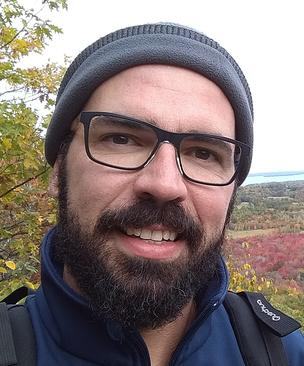
\includegraphics[width=1.0\columnwidth]{Vitor_CV_4.jpg}\\[\baselineskip] % Your photo
\small % Smaller font size
Vitor Vasconcelos Araújo Silva
\url{vitors.vasconcelos@gmail.com} \\ % Your email address
\url{github.com/vitorvas} \\ % Your URL
+34 634 807 860\\ % Your phone number
Born 10/22/1977 \\
\Sep % Some whitespace
\textbf{Address} \\
Calle San Clemente 1, Piso 9, Puerta 4 \\
Santa Cruz de Tenerife, 30008 \\ % Address 2
Spain \\ % Address 3
\vfill % Whitespace under this block to push it up under the photo
\end{flushright}
}

%----------------------------------------------------------------------------------------

\begin{document}

\userinformation % Print your information in the left column

\framebreak % End of the first column

%----------------------------------------------------------------------------------------
%	HEADING
%----------------------------------------------------------------------------------------

\cvheading{Vitor Vasconcelos Araújo Silva} % Large heading - your name

\cvsubheading{Computer Scientist} % Subheading - your occupation/specialization

%----------------------------------------------------------------------------------------
%	ABOUT ME
%----------------------------------------------------------------------------------------

\aboutme{About Me}{Computer scientist of formation, I also had training on radiation protection and nuclear safety and security. I have experience in Linux
  environment use, installation and management and also in computer programming. Since 2011 I work as part of a mixed group of Mechanical and Electrical
  engineers, being the only Computer Scientist. Most of the group activities are related to thermal-hydraulics and neutronics simulation of nuclear reactors. My current activities are strongly related to software development
aimed at multiphysics calculations and Linux systems administration. I am also the system administrator of a small HPC system of 9 nodes (180 processors). \textbf{(In sabbatical leave during 2020)}}

%----------------------------------------------------------------------------------------
%	EDUCATION
%----------------------------------------------------------------------------------------

\CVSection{Education}

%------------------------------------------------


\CVItem{2011 - 2016, Universidade Federal de Minas Gerais - UFMG}{D.Sc in Nuclear Sciences - Nuclear Engineering}\\
\CVItem{Sep 2010 - Dec 2010, Universidad de Buenos Aires - UBA}{Postgraduate Certificate in Nuclear Safety (345h)}\\
\CVItem{Mar 2010 - Sep 2010, Universidad de Buenos Aires - UBA}{Postgraduate Certificate in Radiation Protection and Radiation Sources Safety (700h)}\\
\CVItem{2003 - 2006, Universidade Federal de Rio de Janeiro - UFRJ}{M.Sc in Systems and Computational Engineering - Image Processing and Computer Graphics}\\
\CVItem{1999 - 2002, Universidade Federal de Minas Gerais - UFMG}{B.Sc in Computer Science}\\

%------------------------------------------------

\Sep % Extra whitespace after the end of a major section

%----------------------------------------------------------------------------------------
%	NEW PAGE DELIMITER
%	Place this block wherever you would like the content of your CV to go onto the next page
%----------------------------------------------------------------------------------------

\clearpage % Start a new page

\userinformation % Print your information in the left column

\framebreak % End of the first column


%----------------------------------------------------------------------------------------
%	EXPERIENCE
%----------------------------------------------------------------------------------------

\CVSection{Experience}

%------------------------------------------------

\CVItem{April 2009 - present, \textit{Senior Technologist}, Nuclear Technology Development Center (CDTN) [Belo Horizonte, BRAZIL]}{
  Detailed achievements:\\
  \textbf{at Radiations Dosimetry Department (Apr 2009 - Jul 2011)}
  \begin{itemize}
  \item  Management of film based dosimetry software and database of CDTN.
  \end{itemize}
  \textbf{at Nuclear Reactors Technology Department (Aug 2011 - today)}
  \begin{itemize}
  \item Linux administrator at Thermal-hydraulics CFD laboratory.
  \item Computational Fluid Dynamics (CFD) modelling of TRIGA IPR-R1 reactor and neutronics modelling
    of TRIGA IPR-R1 reactor using \textit{Serpent} Monte Carlo code.
  \item Free software development using \textit{OpenFOAM} CFD framework.
  \item \textit{OpenFOAM} CFD coupling with deterministic finite volumes free nuclear code \textit{milonga}.
  \item Undergraduate students advisor on software development.
  \item Radiation protection plan of TRIGA IPR-R1 reactor updating.
  \item Manager and system administrator of Department's new cluster system (9 nodes, 180 cores),
    CentOS Linux each node equipped with graphics processing units (GPU).
  \item Recently involved in studies of feasibility of extending Monte Carlo software to use graphical processing
    units (GPUs).
  \end{itemize}
}


%------------------------------------------------

\CVItem{Dec 2006 - Nov 2008, \textit{Software Engineer at research team \textit{QGAR}}, INRIA Grand'Est, [Nancy, FRANCE]}{
  Detailed achievements:
  \begin{itemize}
  \item Multi-platform compilation scripts for the pattern recognition and image analysis tool \textit{QGAR}.
  \item Re-writing \textit{Qt} library dependent code to comply with new API (C++).
  \item \textit{QGAR} Graphics User Interface maintenance and development (C++ and Qt).
  \item Incorporation of new algorithms to \textit{QGAR} tool.
  \end{itemize}
}

\CVItem{Sep 2002 - Nov 2006, \textit{Junior Technologist}, National Nuclear Energy Commission (CNEN) [Rio de Janeiro, BRAZIL]}{
  Detailed achievements:
  \begin{itemize}
  \item Linux electronic mail administrator (Sendmail and Postfix).
  \item Microsoft ASP systems development and maintenance.
  \item Neutrongraphy image processing algorithm development.
  \end{itemize}
}
%------------------------------------------------

\Sep % Extra whitespace after the end of a major section

%----------------------------------------------------------------------------------------
%	NEW PAGE DELIMITER
%	Place this block wherever you would like the content of your CV to go onto the next page
%----------------------------------------------------------------------------------------


\clearpage % Start a new page
\userinformation % Print your information in the left column
\framebreak % End of the first column


%----------------------------------------------------------------------------------------
%	COMMUNICATION SKILLS
%----------------------------------------------------------------------------------------

\CVSection{Language Skills}

%------------------------------------------------

\CVItem{Portuguese}{\textit{Mother Language}.}\\
%\CVItem{English}{\textit{Fluent}.}\\
\CVItem{English, French and Spanish}{ \textit{Read, Speak and Understand. Good written skills}.}\\

%------------------------------------------------

\Sep % Extra whitespace after the end of a major section

%----------------------------------------------------------------------------------------
%	SKILLS
%----------------------------------------------------------------------------------------

\CVSection{Software Development Skills}

%------------------------------------------------

\CVItem{Programming}
 {\begin{tabular}{p{0.15\textwidth} p{0.15\textwidth} p{0.15\textwidth} p{0.15\textwidth}}
 \textbf{Experienced:} & & &\\          
 \bluebullet C &  \bluebullet C++ & \bluebullet Linux & \bluebullet bash\\
 \textbf{Intermediary:} & & &\\          
 \bluebullet MPI &  \bluebullet OpenMP & \bluebullet Perl & \bluebullet Python\\
 \textbf{Basic:} & & &\\          
 \bluebullet SYCL &  \bluebullet OpenCL & \bluebullet CUDA & \\
\end{tabular}}
       
       %------------------------------------------------

\CVItem{Most used Computer Software, Libraries and Tools}
{\begin{tabular}{p{0.325\textwidth} p{0.3\textwidth} }
    \bluebullet Serpent Monte Carlo &  \bluebullet OpenFOAM \\
    \bluebullet ParaView & \bluebullet Git\\
    \bluebullet emacs & \bluebullet VTK\\
    \bluebullet LaTeX & \bluebullet Valgrind\\ %\LaTeX nao imprime legal
\end{tabular}}

%------------------------------------------------

\Sep % Extra whitespace after the end of a major section


%----------------------------------------------------------------------------------------
%	SKILLS
%----------------------------------------------------------------------------------------

\CVSection{Short Courses}

%------------------------------------------------

\CVItem{2007}{\textit{Calcul Numérique Certifié [Rigorous Numerics] (16h).
Institut National de Recherche en Informatique et en Automatique - LORIA/INRIA, Nancy, France}.}\\
\CVItem{2010}{\textit{Geant4 Tutorial (40h).
Centre Européen pour la Recherche Nucléaire, CERN, Geneva, Swizterland}.}\\
\CVItem{2015}{\textit{Workshop on Accelerated High-Performance Computing in Computational Sciences (80h).
    The Abdus Salam International Centre for Theoretical Physics, ICTP, Trieste, Italy}.}\\
\CVItem{2018}{\textit{6th Workshop on Collaborative Scientific Software Development and Management of Open Source Scientific Packages (80h).
    Sharif University of Technology, Tehran, Iran} (ICTP Sponsored).}\\
\CVItem{2019}{\textit{4th IAEA Training Workshop on Advanced Use of Neutron Imaging for Research and Applications (30h).
    Korea Atomic Energy Research Institute, Daejeon, Republic of Korea} (IAEA Sponsored).}\\

%------------------------------------------------

\Sep % Extra whitespace after the end of a major section

%----------------------------------------------------------------------------------------
%	NEW PAGE DELIMITER
%	Place this block wherever you would like the content of your CV to go onto the next page
%----------------------------------------------------------------------------------------

\clearpage % Start a new page

\userinformation % Print your information in the left column

\framebreak % End of the first column

%------------------------------------------------

%----------------------------------------------------------------------------------------
%	PUBLICATIONS
%----------------------------------------------------------------------------------------

\CVSection{Main publications}

\CVItem{Vasconcelos, Vitor; Santos, André; Campolina, Daniel; Theler, Germán; Pereira, Claubia}{\textit{Coupled unstructured fine-mesh neutronics and thermal-hydraulics methodology using open software: A proof-of-concept. ANNALS OF NUCLEAR ENERGY, v. 115, p. 173-185, 2018.}}

%\CVItem{Campolina, Daniel; da Costa, Antônio Carlos L.; Andrade, Edison P.; Santos, André A.C.; Vasconcelos, Vitor}{\textit{Neutronic analysis of the fuel loaded irradiation loop device of the RMB Multipurpose Brazilian Reactor. PROGRESS IN NUCLEAR ENERGY, v. 104, p. 109-116, 2018.}}

\CVItem{Santiago Vieira, Tiago A.; Barros, Graiciany P.; Campolina, Daniel; Vasconcelos, Vitor; Campagnole dos Santos, André A.}{\textit{Study of a fine-mesh 1:1 Computational Fluid Dynamics–Monte Carlo neutron transport coupling method with discretization uncertainty estimation. ANNALS OF NUCLEAR ENERGY, v. 148, p. 107718, 2020.}}

%\CVItem{}{\texit{Fuel breeding and waste burnup capabilities of an ADS using thorium and reprocessed fuels. INTERNATIONAL JOURNAL OF ENERGY RESEARCH, \textbf{accepted, to appear}, 2020.}}

\CVItem{Silva, V. V. A.; Barros, G. P.; Santos, A. A. C.; Campolina, D. A. M.}{\textit{The LTHN Cluster. In: International Nuclear Atlantic Conference (INAC), 2019, Santos, SP, Brazil. Nuclear New Horizons: Fueling our Future.}}

\CVItem{Silva, V. V. A.; Santos, A. A. C.; Cunha, R. O.}{\textit{Professional cluster management by a small scientific team: challenges, solutions and perspectives. In: International Nuclear Atlantic Conference (INAC), 2017, Belo Horizonte, MG, Brazil. Nuclear Energy for National Projects.}}

%\CVItem{Silva, V. V. A.; Santos, A. A. C.; Bernal, A.; Miró; R.; Verdú, G.; Pereira, C.}{\textit{Finite Volume thermal-hydraulics and neutronics coupled calculations.
%    ICAPP - International Congress on Advances in Nuclear Power Plants, 2015, Nice. Proceedings of ICAPP 2015.}}

%----------------------------------------------------------------------------------------
%	AWARDS
%----------------------------------------------------------------------------------------

\CVSection{Awards}

%------------------------------------------------

\CVItem{2013, \textit{CAPES Sandwich Scholarship}, Universidad Politècnica de València [Valencia, SPAIN]}{Brazilian government funding for one year doctoral studies abroad.}

%------------------------------------------------

\Sep % Extra whitespace after the end of a major section


%----------------------------------------------------------------------------------------
%	INTERESTS
%----------------------------------------------------------------------------------------

\CVSection{Interests}

%------------------------------------------------

\CVItem{Professional}{Scientific computing and visulization, free software development, GPU programming, software parallelization techniques, HPC, Linux and heterogeneus computing and programming (SYCL), neutron imaging.}

%------------------------------------------------

\CVItem{Personal}{Hiking, traveling, swimming and reading.}

%------------------------------------------------

\Sep % Extra whitespace after the end of a major section

%----------------------------------------------------------------------------------------

\end{document}
